\documentclass[a4paper,12pt,obeyspaces,spaces,hyphens]{article}

\def \trainingtype{online}
\def \agendalanguage{french}

\input{agenda/yocto.inc}

\usepackage{agenda}

\begin{document}

\feshowtitle

\feagendasummaryitem{Titre}{
  {\bf \trainingtitle{}}
}
\feagendasummaryitem{Objectifs\newline opérationnels}{
  \traininggoals{}
}
\feagendasummaryitem{Durée}{
  \feshowduration{}
}
\onlinepedagogics
\feagendasummaryitem{Formateur}{
  \trainers{}
}
\feagendasummaryitem{Langue}{
  \traininglanguages{}
}
\feagendasummaryitem{Public visé}{
  \trainingaudience{}
}
\feagendasummaryitem{Pré-requis}{
  \trainingprerequisites{}
}
\feagendasummaryitem{Équipement nécessaire}{
  \requiredequipment{}
}
\certificate{}
\disabilities{}

\feagendatwocolumn
{Matériel, première option}
{
  Carte BeagleBone Black
  \begin{itemize}
  \item Un processeur ARM AM335x de Texas Instruments (à base de
    Cortex-A8), avec accélération 3D, etc.
  \item 512 Mo de RAM
  \item 2 Go de stockage eMMC embarqué sur la carte
	\newline(4 Go avec la révision C)
  \item USB hôte et device
  \item Sortie HDMI
  \item Connecteurs à 2 x 46 broches, pour accéder aux UARTs, aux
        bus SPI, aux bus I2C, et à d'autres entrées/sorties du
        processeur.
  \end{itemize}
}{}
{
  \begin{center}
    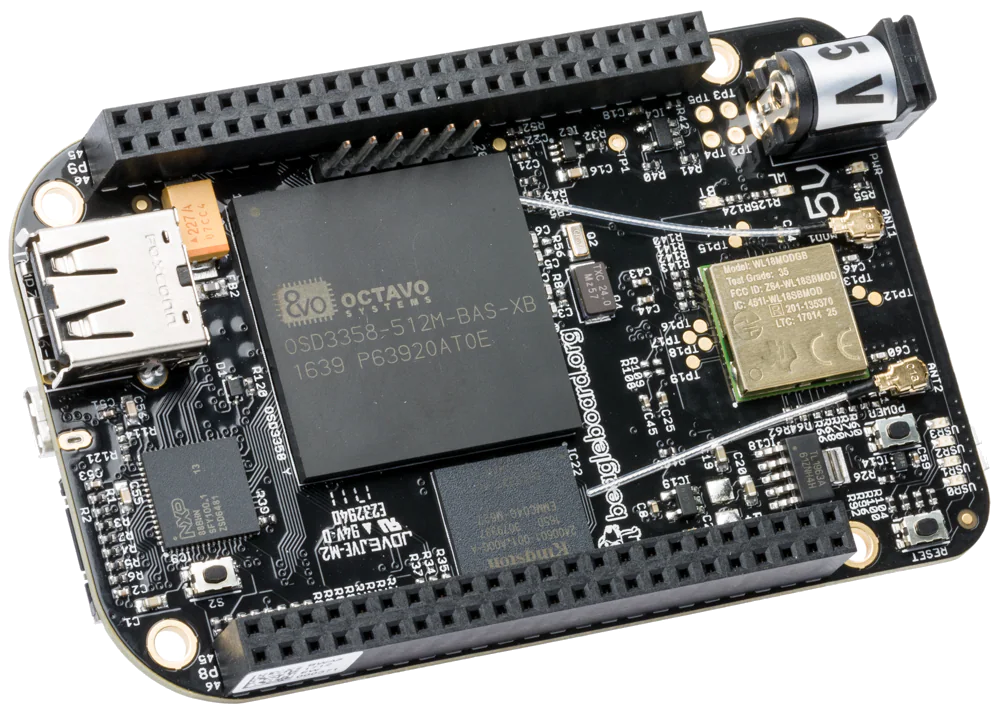
\includegraphics[width=5cm]{../slides/beagleboneblack-board/beagleboneblack.png}
  \end{center}
}

\feagendatwocolumn
{Matériel, deuxième option}
{
  Une de ces cartes de STMicroelectronics: {\bf
  STM32MP157A-DK1}, {\bf STM32MP157D-DK1}, {\bf STM32MP157C-DK2} ou
  {\bf STM32MP157F-DK2}
  \begin{itemize}
  \item Processeur STM32MP157, double Cortex-A7, de STMicroelectronics
  \item Alimentée par USB
  \item 512 Mo DDR3L RAM
  \item Port Gigabit Ethernet port
  \item 4 ports hôte USB 2.0
  \item 1 port USB-C OTG
  \item 1 connecteur Micro SD
  \item Debugger ST-LINK/V2-1 sur la carte
  \item Connecteurs compatibles Arduino Uno v3
  \item Codec audio
  \item Divers: boutons, LEDs
  \item Écran LCD tactile (uniquement sur cartes DK2)
  \end{itemize}
}{}
{
  \begin{center}
    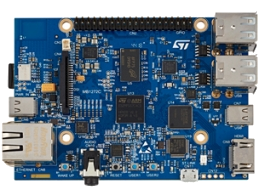
\includegraphics[width=5cm]{../slides/discovery-board-dk1/discovery-board-dk1.png}
  \end{center}
}

\section{1\textsuperscript{ère} demi-journée}

\feagendaonecolumn
{Cours - Introduction aux outils de compilation de systèmes Linux embarqué}
{
  \begin{itemize}
  \item Vue d'ensemble de l'architecture d'un système Linux embarqué
  \item Méthodes pour compiler un système de fichiers
  \item Utilité des outils de compilation
  \end{itemize}
}

\feagendatwocolumn
{Cours - Vue d'ensemble de Yocto Project et du système de référence Poky}
{
  \begin{itemize}
  \item Organisation des sources du projet
  \item Création d'un système de fichiers avec Yocto Project
  \end{itemize}
}
{Démo - 1\textsuperscript{ère} compilation avec Yocto Project}
{
  \begin{itemize}
  \item Téléchargement du système de référence Poky
  \item Compilation d'une image système
 \end{itemize}
}

\newpage
\feagendatwocolumn
{Cours - Utilisation de Yocto Project - Notions de base}
{
  \begin{itemize}
  \item Structure des fichiers générés
  \item Flasher et installer l'image du système
  \end{itemize}
}
{Démo - Flasher et booter}
{
  \begin{itemize}
  \item Flasher et booter l'image du système sur la carte
  \end{itemize}
}

\section{2\textsuperscript{ème} demi-journée}

\feagendatwocolumn
{Cours - Utilisation de Yocto Project - Utilisation avancée}
{
  \begin{itemize}
  \item Configuration de la compilation
  \item Personnalisation de la sélection de paquetages
  \end{itemize}
}
{Démo - Utilisation de NFS et configuration de la compilation}
{
  \begin{itemize}
  \item Configurer la carte pour démarrer via NFS
  \item Apprendre à utiliser le mécanisme \code{PREFERRED_PROVIDER}
  \end{itemize}
}
\\

\feagendatwocolumn
{Cours - Écriture de recettes - Fonctionnalités de base}
{
  \begin{itemize}
  \item Écriture d'une recette minimale
  \item Ajout de dépendances
  \item Organisation du développement avec {\em bitbake}
  \end{itemize}
}
{Démo - Ajouter la compilation d'une application}
{
  \begin{itemize}
  \item Création d'une recette pour {\em nInvaders}
  \item Ajout d'{\em nInvaders} à l'image finale
  \end{itemize}
}

\feagendaonecolumn
{Cours - Écriture de recettes - Fonctionnalités avancées}
{
  \begin{itemize}
  \item Extension et redéfinition de recettes
  \item Rajouter des étapes au processus de compilation
  \item Familiarisation avec les classes
  \item Analyse d'exemples
  \item Logs
  \item Mise au point des dépendances
  \end{itemize}
}

\section{3\textsuperscript{ème} demi-journée}

\feagendatwocolumn
{Cours - Layers}
{
  \begin{itemize}
  \item Ce que sont les {\em layers}
  \item Où trouver les {\em layers}
  \item Création d'un {\em layer}
  \end{itemize}
}
{Démo - Écriture d'un layer}
{
  \begin{itemize}
  \item Apprendre à écrire un {\em layer}
  \item Ajouter le {\em layer} à la compilation
  \item Inclure {\em nInvaders} dans le nouveau {\em layer}
  \end{itemize}
}

\feagendatwocolumn
{Cours - Écriture d'un BSP}
{
  \begin{itemize}
  \item Extension d'un BSP existant
  \item Ajout d'une nouvelle machine
  \item Chargeurs de démarrage
  \item Linux et la recette linux-yocto
  \item Ajouter un type d'image personnalisé
  \end{itemize}
}
{Démo - Mise en oeuvre de modifications du noyau}
{
  \begin{itemize}
  \item Extension de la recette pour le noyau pour ajouter le pilote
        pour le Nunchuk
  \item Configurer le noyau pour compiler le pilote du Nunchuk
  \item Jouer à {\em nInvaders}
  \end{itemize}
}

\section{4\textsuperscript{ème} demi-journée}

\feagendatwocolumn
{Cours - Création d'une image sur mesure}
{
  \begin{itemize}
  \item Écriture d'une recette d'image
  \item Ajouter des utilisateurs et des groupes
  \item Ajouter une configuration personnalisée
  \item Écrire et utiliser des groupes de recettes de paquetages
  \end{itemize}
}
{Démo - Création d'une image sur mesure}
{
  \begin{itemize}
  \item Écrire une recette d'image personnalisée
  \item Ajouter {\em nInvaders} à l'image sur mesure
  \end{itemize}
}
\feagendatwocolumn
{Cours - Création et utilisation d'un SDK}
{
  \begin{itemize}
  \item Comprendre l'utilité d'un SDK pour le développeur d'applications
  \item Construire un SDK pour l'image sur mesure
  \end{itemize}
}
{Démo - Expérimentations avec le SDK}
{
  \begin{itemize}
  \item Construction d'un SDK
  \item Utilisation du SDK de Yocto Project
  \end{itemize}
}

\feagendaonecolumn
{Questions / réponses}
{
  \begin{itemize}
  \item Questions et réponses avec les participants à propos des sujets abordés.
  \item Présentations supplémentaires s'il reste du temps, en fonction des demandes
        de la majorité des participants.
  \end{itemize}
}

\section{Temps supplémentaire possible}

{\em Du temps supplémentaire (jusqu'à 4 heures) pourrait être proposé si le programme ne tenait
     pas en 4 demi-journées, selon le temps passé à répondre aux questions des participants.}

\end{document}
